\documentclass[10pt]{beamer}

\usetheme{metropolis}
\usepackage{appendixnumberbeamer}

% Add graphics path
\usepackage{graphicx}
\graphicspath{ {img/} }

% Animation package
\usepackage{animate}

\usepackage{booktabs}
\usepackage[scale=2]{ccicons}

\usepackage{pgfplots}
\usepgfplotslibrary{dateplot}

% Add connected lines to dot of navigation bar
\makeatletter
\setbeamertemplate{headline}{%
	\begin{beamercolorbox}[colsep=1.5pt]{upper separation line head}
	\end{beamercolorbox}
	\begin{beamercolorbox}{section in head/foot}
		\vskip2pt\insertnavigation{\paperwidth}\vskip2pt
	\end{beamercolorbox}%
	\begin{beamercolorbox}[colsep=1.5pt]{lower separation line head}
	\end{beamercolorbox}
}
\makeatother

\setbeamercolor{section in head/foot}{fg=normal text.bg, bg=structure.fg}

\makeatletter
\def\slideentry#1#2#3#4#5#6{%
	%section number, subsection number, slide number, first/last frame, page number, part number
	\ifnum#6=\c@part\ifnum#2>0\ifnum#3>0%
	\ifbeamer@compress%
	\advance\beamer@xpos by1\relax%
	\else%
	\beamer@xpos=#3\relax%
	\beamer@ypos=#2\relax%
	\fi%
	\hbox to 0pt{%
		\beamer@tempdim=-\beamer@vboxoffset%
		\advance\beamer@tempdim by-\beamer@boxsize%
		\multiply\beamer@tempdim by\beamer@ypos%
		\advance\beamer@tempdim by -.05cm%
		\raise\beamer@tempdim\hbox{%
			\beamer@tempdim=\beamer@boxsize%
			\multiply\beamer@tempdim by\beamer@xpos%
			\advance\beamer@tempdim by -\beamer@boxsize%
			\advance\beamer@tempdim by 1pt%
			\kern\beamer@tempdim
			\global\beamer@section@min@dim\beamer@tempdim
			\hbox{\beamer@link(#4){%
					\usebeamerfont{mini frame}%
					\ifnum\c@section=#1%
					\ifnum\c@subsection=#2%
					\usebeamercolor[fg]{mini frame}%
					\ifnum\c@subsectionslide=#3%
					\ifnum#3=1%
					\usebeamertemplate{mini frame first}%\beamer@minislidehilight%
					\else%
					\usebeamertemplate{mini frame}%\beamer@minislidehilight%
					\fi
					\else%
					\ifnum#3=1%
					\usebeamertemplate{mini frame in current subsection first}%
					\else%
					\usebeamertemplate{mini frame in current subsection}%\beamer@minisliderowhilight%
					\fi
					\fi%
					\else%
					\usebeamercolor{mini frame}%
					%\color{fg!50!bg}%
					\usebeamertemplate{mini frame in other subsection}%\beamer@minislide%
					\fi%
					\else%
					\usebeamercolor{mini frame}%
					%\color{fg!50!bg}%
					\usebeamertemplate{mini frame in other subsection}%\beamer@minislide%
					\fi%
				}}}\hskip-10cm plus 1fil%
			}\fi\fi%
			\else%
			\fakeslideentry{#1}{#2}{#3}{#4}{#5}{#6}%
			\fi\ignorespaces
		}
		\makeatother
		
		\defbeamertemplate{mini frame}{scaled circle}[1]
		{%
			\begin{pgfpicture}{0pt}{0pt}{#1 * 0.1cm}{#1 * 0.1cm}
				\pgfsetlinewidth{#1 * 0.4pt}
				\pgfpathmoveto{\pgfpoint{0cm}{#1 * 0.05cm}} 
				\pgfpathlineto{\pgfpoint{#1 * -0.04cm}{#1 * 0.05cm}} 
				\pgfpathcircle{\pgfpoint{#1 * 0.05cm}{#1 * 0.05cm}}{#1 * 0.05cm}
				\pgfusepath{fill,stroke}
			\end{pgfpicture}%
		}
		[action]
		{
			\newlength{\myminiframesize}
			\setlength{\myminiframesize}{0.14cm}
			\newlength{\myminiframeoffset}
			\setlength{\myminiframeoffset}{0.03cm}
			\setbeamersize{mini frame size=#1\myminiframesize,mini frame offset=#1\myminiframeoffset}
		}
		
		\defbeamertemplate{mini frame first}{scaled circle}[1]
		{%
			\begin{pgfpicture}{0pt}{0pt}{#1 * 0.1cm}{#1 * 0.1cm}
				\pgfsetlinewidth{#1 * 0.4pt}
				\pgfpathcircle{\pgfpoint{#1 * 0.05cm}{#1 * 0.05cm}}{#1 * 0.05cm}
				\pgfusepath{fill,stroke}
			\end{pgfpicture}%
		}
		
		
		\defbeamertemplate{mini frame in current section}{scaled circle}[1]
		{%
			\begin{pgfpicture}{0pt}{0pt}{#1 * 0.1cm}{#1 * 0.1cm}
				\pgfsetlinewidth{#1 * 0.4pt}
				\pgfpathmoveto{\pgfpoint{0cm}{#1 * 0.05cm}} 
				\pgfpathlineto{\pgfpoint{#1 * -0.04cm}{#1 * 0.05cm}} 
				\pgfpathcircle{\pgfpoint{#1 * 0.05cm}{#1 * 0.05cm}}{#1 * 0.05cm}
				\pgfusepath{stroke}
			\end{pgfpicture}%
		}
		
		\defbeamertemplate{mini frame in other section}{scaled circle}[1]
		{%
			\color{fg!50!bg}
			\begin{pgfpicture}{0pt}{0pt}{#1 * 0.1cm}{#1 * 0.1cm}
				\pgfsetlinewidth{#1 * 0.4pt}
				\pgfpathcircle{\pgfpoint{#1 * 0.05cm}{#1 * 0.05cm}}{#1 * 0.05cm}
				\pgfusepath{stroke}
			\end{pgfpicture}%
		}
		
		\defbeamertemplate{mini frame in current subsection}{scaled circle}[1]
		{%
			\begin{pgfpicture}{0pt}{0pt}{#1 * 0.1cm}{#1 * 0.1cm}
				\pgfsetlinewidth{#1 * 0.4pt}
				\pgfpathmoveto{\pgfpoint{0cm}{#1 * 0.05cm}} 
				\pgfpathlineto{\pgfpoint{#1 * -0.04cm}{#1 * 0.05cm}} 
				\pgfpathcircle{\pgfpoint{#1 * 0.05cm}{#1 * 0.05cm}}{#1 * 0.05cm}
				\pgfusepath{stroke}
			\end{pgfpicture}%
		}
		
		\defbeamertemplate{mini frame in current subsection first}{scaled circle}[1]
		{%
			\begin{pgfpicture}{0pt}{0pt}{#1 * 0.1cm}{#1 * 0.1cm}
				\pgfsetlinewidth{#1 * 0.4pt}
				\pgfpathcircle{\pgfpoint{#1 * 0.05cm}{#1 * 0.05cm}}{#1 * 0.05cm}
				\pgfusepath{stroke}
			\end{pgfpicture}%
		}
		
		\defbeamertemplate{mini frame in other subsection}{scaled circle}[1]
		{%
			\color{fg!50!bg}
			\begin{pgfpicture}{0pt}{0pt}{#1 * 0.1cm}{#1 * 0.1cm}
				\pgfsetlinewidth{#1 * 0.4pt}
				\pgfpathcircle{\pgfpoint{#1 * 0.05cm}{#1 * 0.05cm}}{#1 * 0.05cm}
				\pgfusepath{stroke}
			\end{pgfpicture}%
		}
		
		\setbeamertemplate{mini frame}[scaled circle]{0.7}
		\setbeamertemplate{mini frame first}[scaled circle]{0.7}
		\setbeamertemplate{mini frame in current section}[scaled circle]{0.7}
		\setbeamertemplate{mini frame in current subsection}[scaled circle]{0.7}
		\setbeamertemplate{mini frame in current subsection first}[scaled circle]{0.7}
		\setbeamertemplate{mini frame in other section}[scaled circle]{0.7}
		\setbeamertemplate{mini frame in other subsection}[scaled circle]{0.7}

\title{Sampling with Markov Chain Monte Carlo}
\subtitle{A look on efficiency and why it is important}
\date{\today}
\author{Quang Ha}
% \institute{Boston University}
% \titlegraphic{\hfill\includegraphics[height=1.5cm]{logo.pdf}}

\begin{document}

% Make the title	
\maketitle

% Table of content
\begin{frame}[plain]{Table of contents}
	\setbeamertemplate{section in toc}[sections numbered]
	\tableofcontents[hideallsubsections]
\end{frame}	

% A brief introduction
\section{Introduction}
\subsection{Definition}

\begin{frame}
	\frametitle{What is Markov Chain Monte Carlo?}
	\begin{itemize}
		\item \textbf{Monte Carlo} is broad class of computational algorithms that rely on repeated random sampling to obtain numerical results. \tiny{Wiki}. \normalsize
		\item \textbf{Markov chain} are random variables having the property that, given the present, the future is conditionally independent of the past. \tiny{Wiki}. \normalsize
			\begin{equation*}
				P(X_{n+1}|X_{n}, X_{n-1}, \cdots, X_0) = P(X_{n+1}|X_{n})
			\end{equation*}
		\item \textbf{Markov Chain Monte Carlo} is a class of algorithms for sampling from a probability distribution based on constructing a Markov chain that has the desired distribution as its equilibrium distribution. \tiny{Wiki}. \normalsize
%		\item Born in the early 1950s in Los Alamos, NM. First implemented on MANIAC computer, built under direction of Nicholas Metropolis. \tiny{Robert et al, 2011}. \normalsize
	\end{itemize}
\end{frame} 

\begin{frame}
	\frametitle{How MCMC works - The landscape perspective}
	\begin{figure}[h]
		\centering
		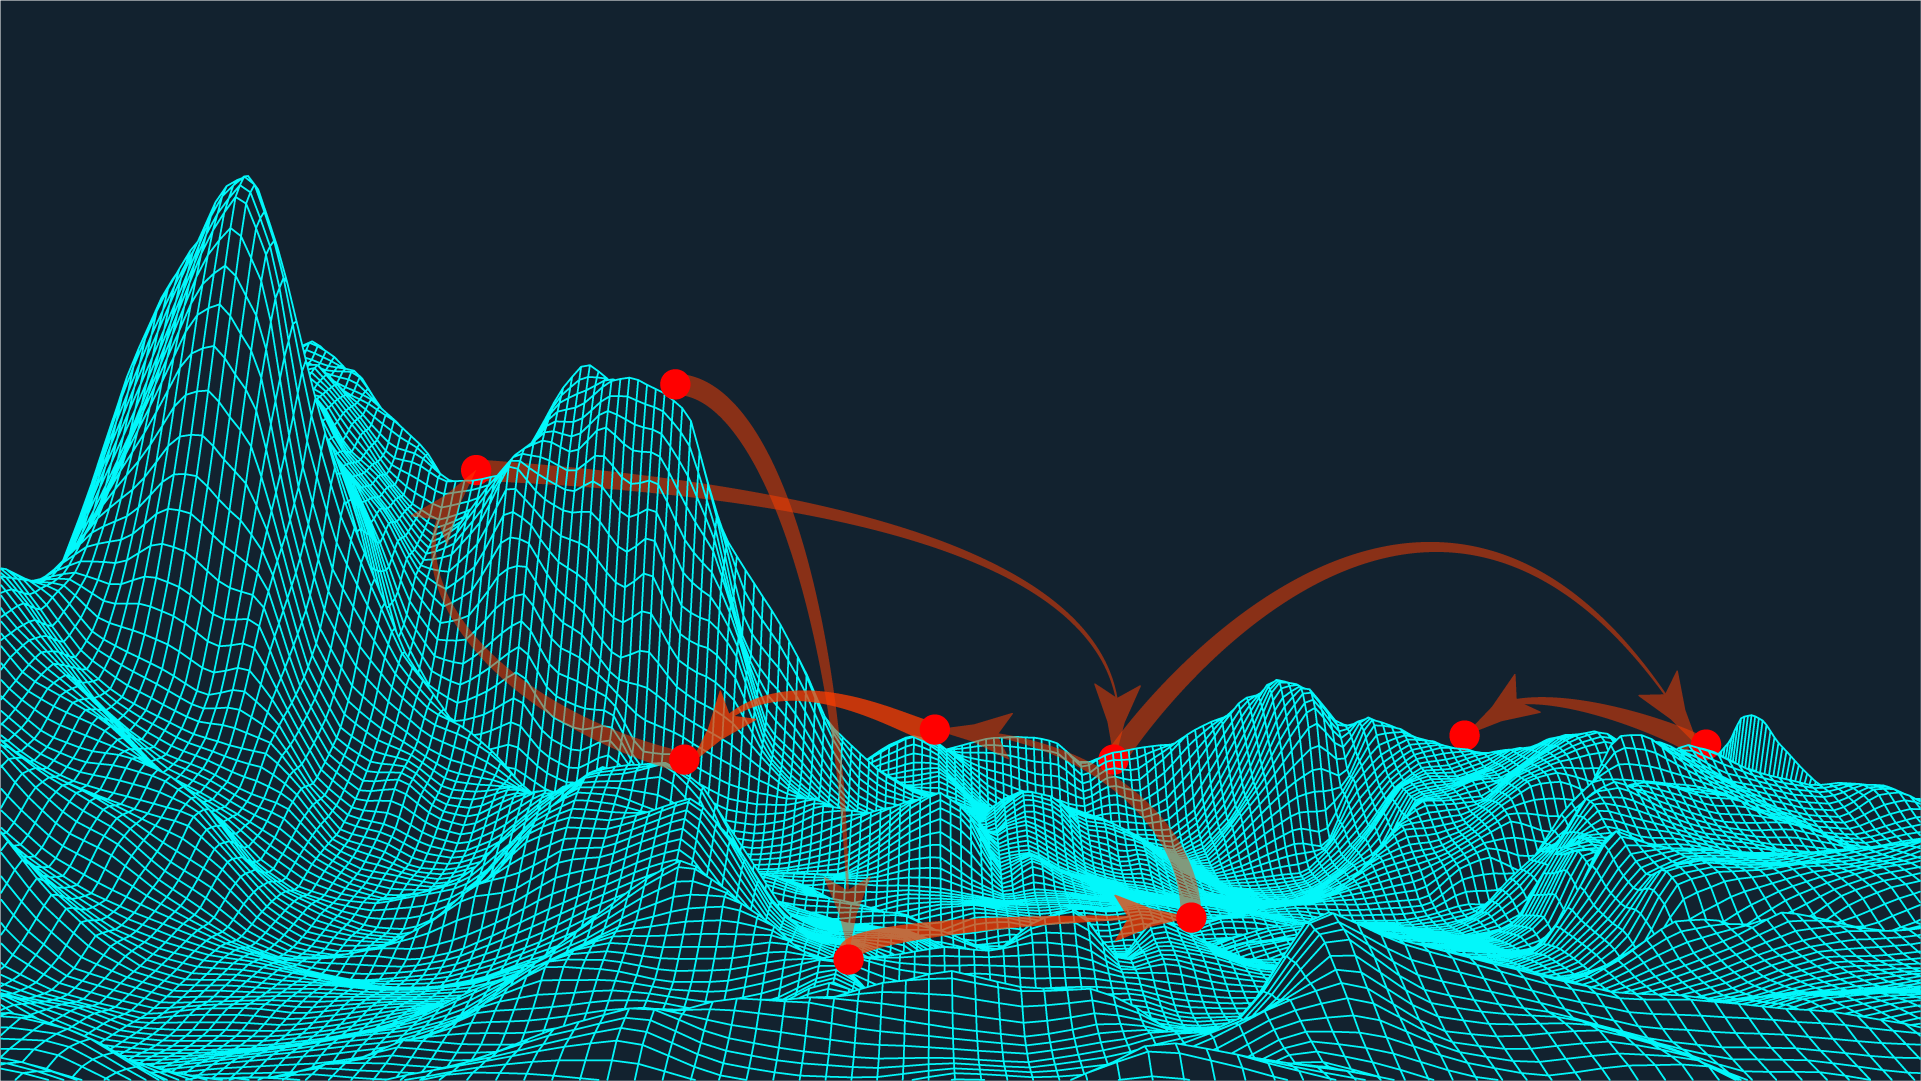
\includegraphics[width=\textwidth]{mountain}
		\caption{Exploring the landscape with random stepping.}
	\end{figure}
\end{frame} 

\begin{frame}
	\frametitle{How MCMC works - More explicit explanation}
	\begin{center}
		\textit{``By collecting a `large' number of pebbles that is likely to come from the mountain, we can `approximately' construct the landscape.''} \\
		\tiny{Davidson-Pilon} \normalsize
	\end{center}
	\begin{itemize}
		\item Start at current position.
		\item \textbf{Propose moving to a new position} - somewhere near you!
		\item Accept/Reject the new position and ask how likely the pebble is from the mountain.
		\begin{itemize}
			\item If it is: Move to the new position.
			\item If not: Stay where you are.
		\end{itemize}
		\item \textbf{After a large number of iterations}, return all \textit{accepted} positions.
	\end{itemize}
\end{frame}

\begin{frame}
	\frametitle{Reasons to use MCMC}
	\begin{itemize}
		\item In most cases, MCMC are used for `black box' system - can only obtained the output given an input.
		\item Preferred method in high-dimension - compared to explicit formula in $N-$dimensions.
		\item Sampling is easy for a uniform distribution in 1D, but not for more complicated pdfs.
		\item Also in high dimensions, method like \textit{rejection-acceptance} will be very inefficient - most of the times we will miss!
	\end{itemize}
\end{frame}

\section{Major challenges}
\subsection{The main problems}

\begin{frame}
	\frametitle{Challenges for MCMC}
	\begin{itemize}
		\item It is important to explore the entire `landscape' - there can be useful information within the `black box'.
		\item The computational cost for getting an output of the `black box` is typically huge - hence rejection rate needs to be minimised!
		\item Sequences of MCMC samples are based on the assumption that the samples are derived from the pdf of interest, and theory guarantees this condition as the number of iterations approaches \textit{infinity}.
		\item Unfortunately, no universal threshold exists across all problems! \tiny{Fonnesbeck, 2014}
	\end{itemize}
\end{frame}

\begin{frame}
	\frametitle{Nostalgic example: HW problem...}
	\begin{figure}[h]
		\centering
		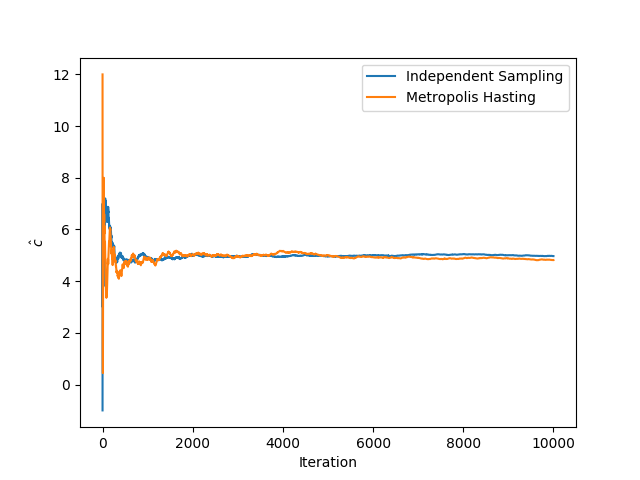
\includegraphics[width=0.8\textwidth]{hw}
		\caption{Example taken from homework 6 - SE/ME 714.}
	\end{figure}	
\end{frame}

\begin{frame}
	\frametitle{Rapid `mixing'}
	\begin{itemize}
		\item `Mixing' indicates how well MCMC samples move through the entire `landscape' of the desired pdf.
		\item In ideal Monte Carlo methods, our samples are expected to be independent. However, this is not the case for Markov chains.
		\item Poor mixing is caused by \textit{inappropiate proposed movings} or \textit{highly-correlated variables.}
		\item Frequently, lack of convergence is caused by poor mixing.
	\end{itemize}
\end{frame}

\begin{frame}
	\frametitle{Poor mixing examples}
	\begin{figure}[h]
		\centering
		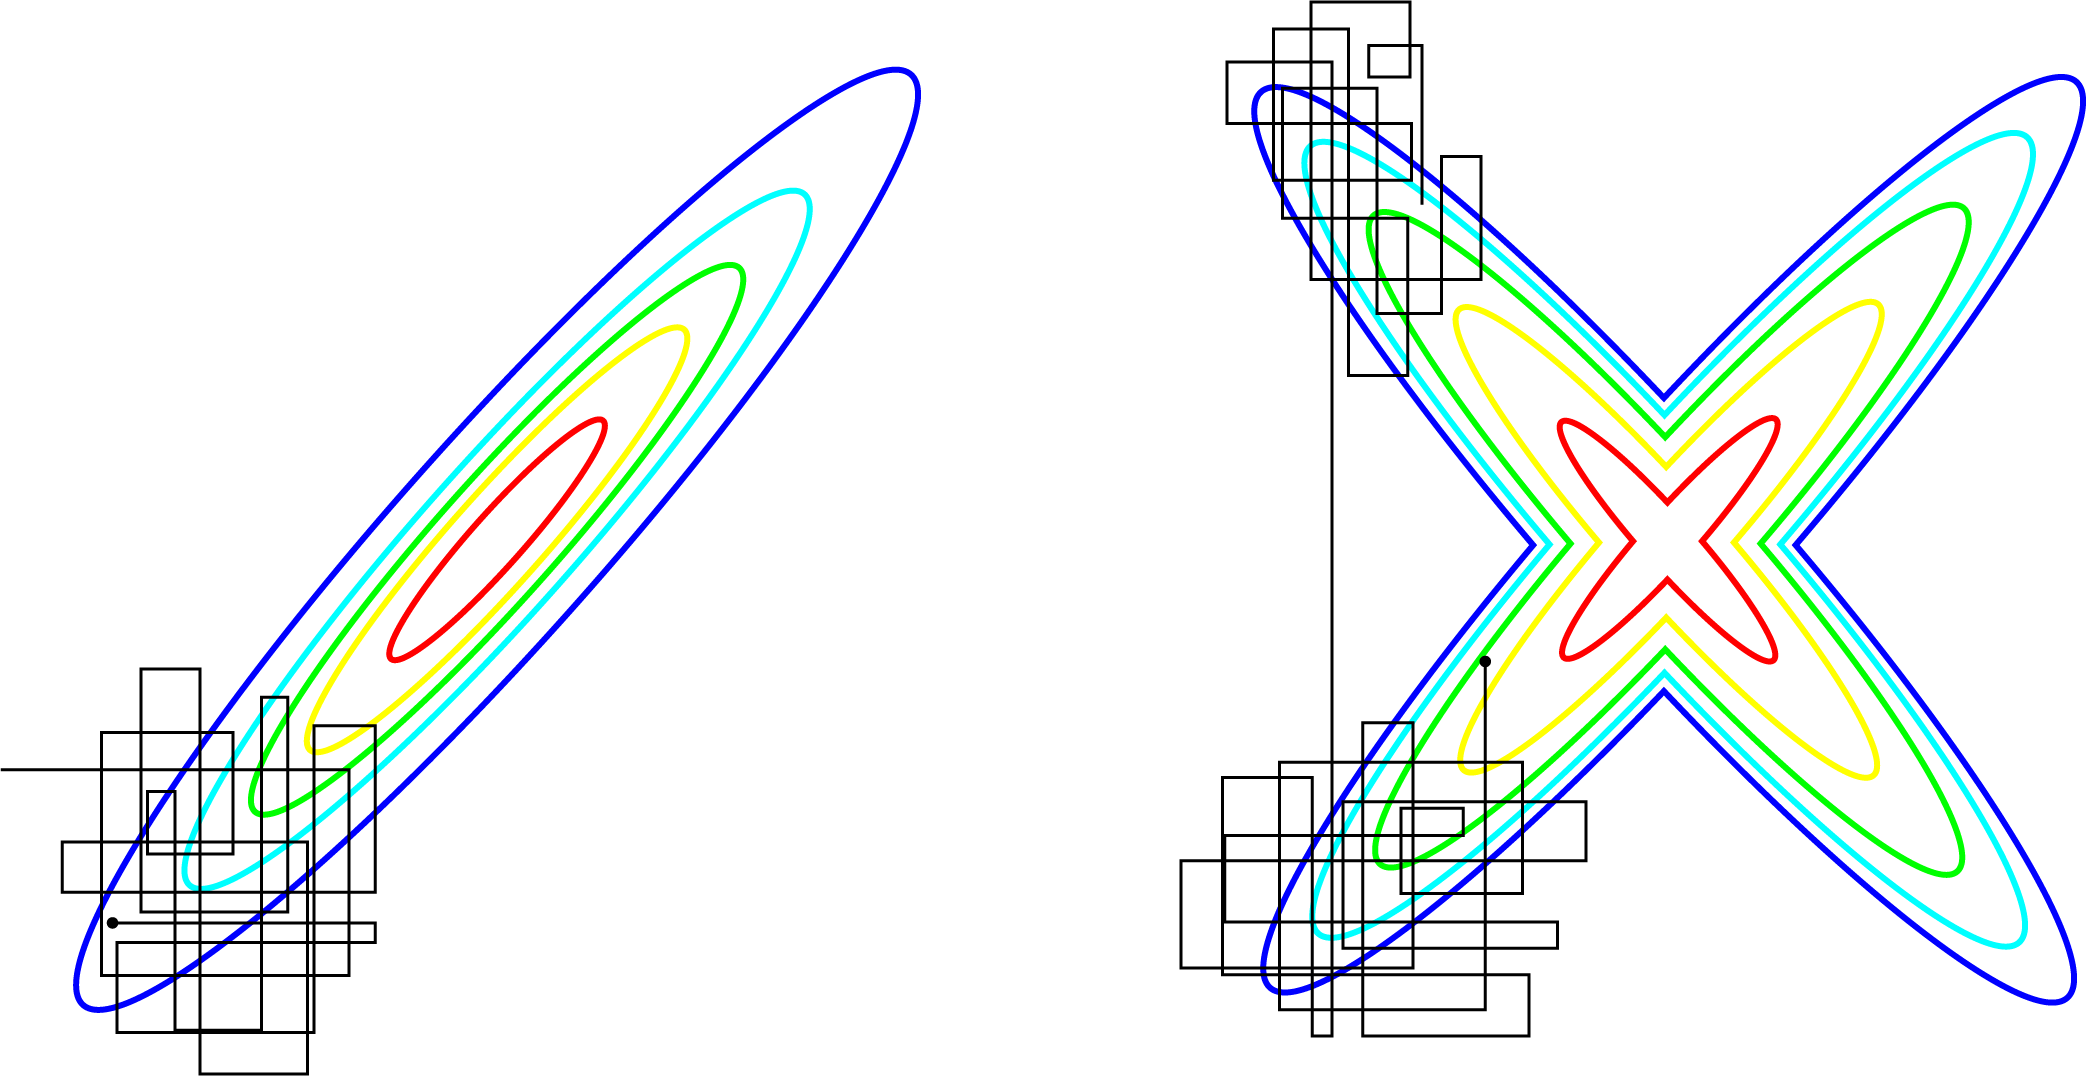
\includegraphics[width=\textwidth]{poor_mixing}
		\caption{Example of poor mixing.}
	\end{figure}	
\end{frame}

\section{Strategies for proposing moves}
\subsection{Proposing moves}

\begin{frame}
	\frametitle{Propose moving to a new position}
	\begin{itemize}
		\item Designing a good strategy for moving/stepping is hard, and it's depends on the desired pdf. 
		\item The proposal move is important to design a rapid mixing MCMC. It is normally built using known `randomness' algorithms.
		\item Known strategies include:
			\begin{itemize}
				\item \textbf{Single-component update}: Gibbs sampling, Component-wise Metropolis Hasting, etc.
				\item \textbf{Adaptive direction sampling}: Hit-and-run, Adaptive direction, etc.
				\item \textbf{Sample from an `easier' distribution}: Importance sampling, etc.
				\item \textbf{Re-sampling from the previous samples}
				\item \textbf{Adopt physical system dynamic}: Hybrid/Hamiltonian MCMC, etc.
			\end{itemize}
			... and many more...
	\end{itemize}
\end{frame}

\begin{frame}
	\frametitle{Single-component update}
	\begin{itemize}
		\item Not many multi-variate distribution to sample from, but we do have several 1D pdfs...
		\item Main drawback: very poor mixing if variables are highly correlated. 
		\item Solution: re-parameterise into independent variables. 
		\item Further problem(!): not as easy for more complicated problems! \tiny{Levine et al, 2003} \normalsize
	\end{itemize}
	\begin{figure}[h]
		\centering
		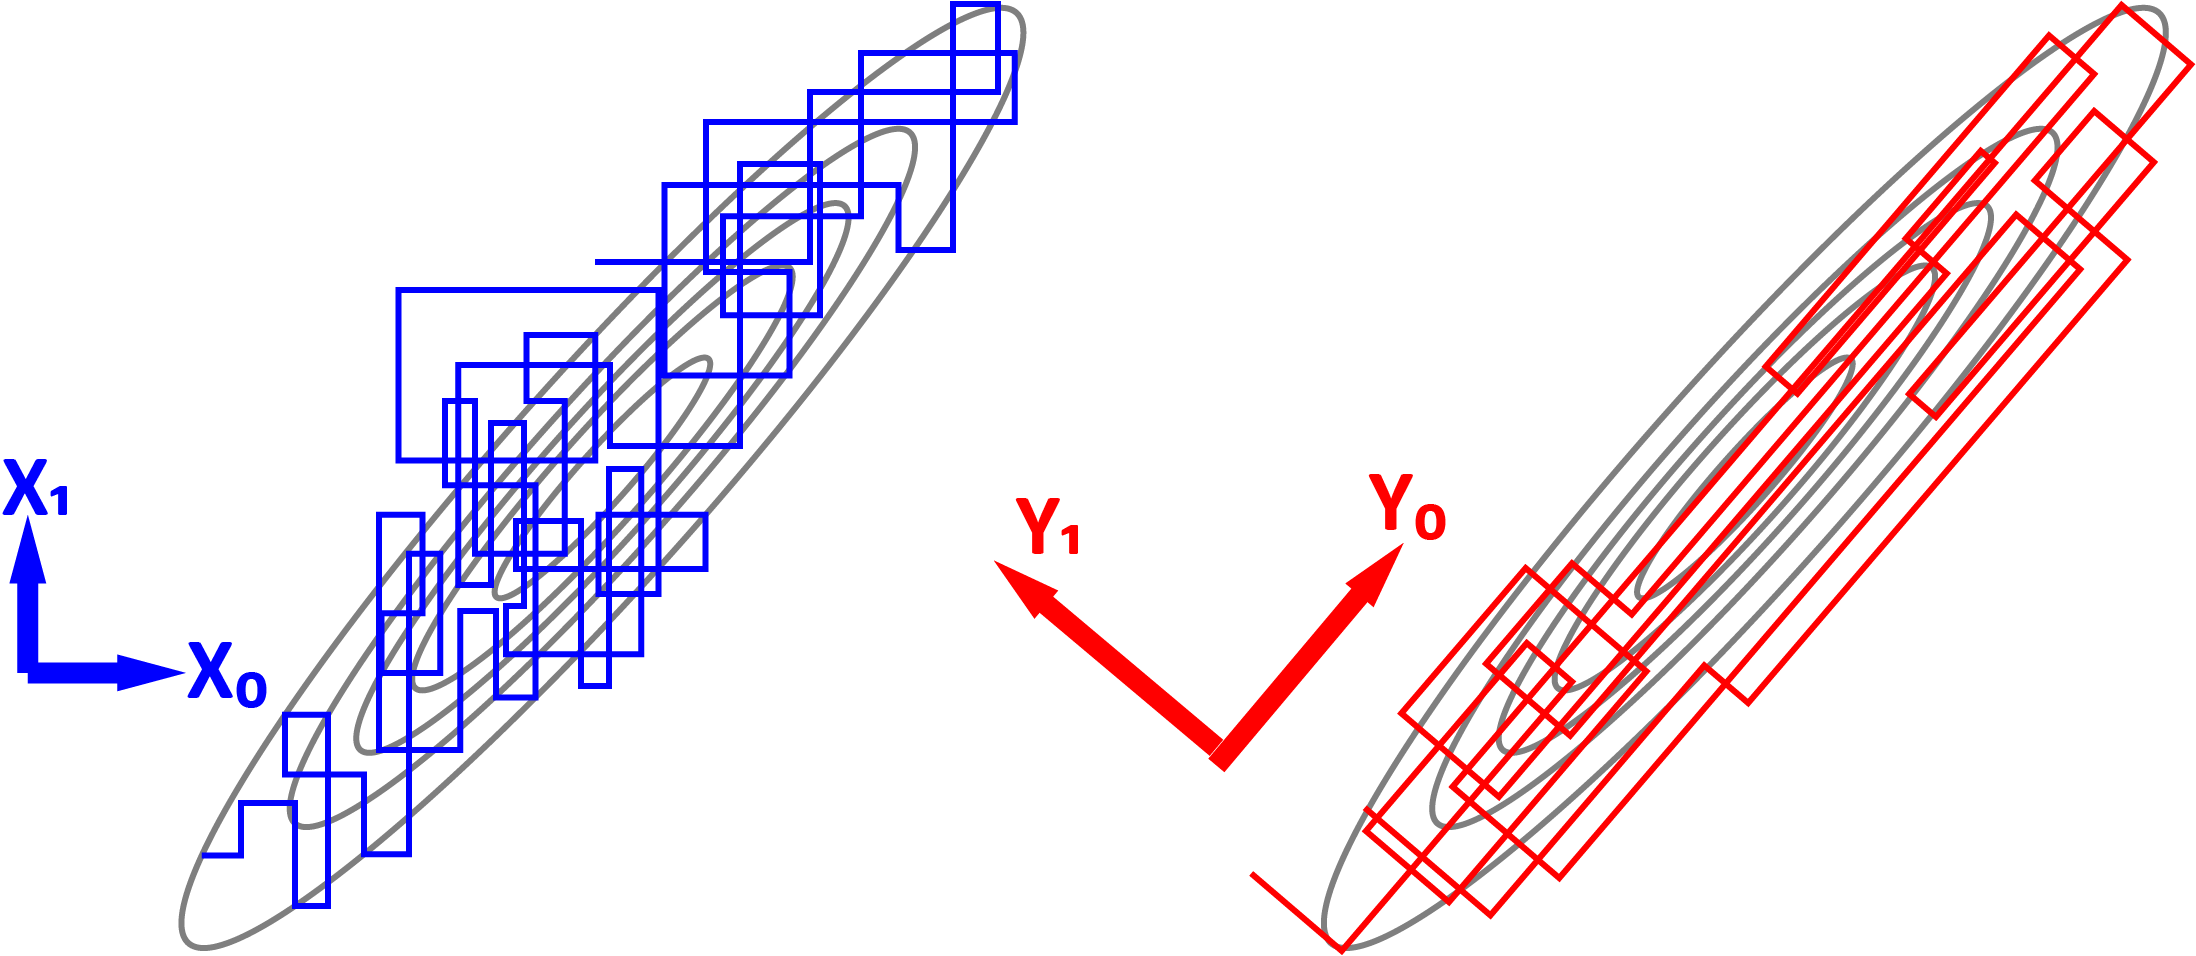
\includegraphics[width=0.8\textwidth]{reparameterisation}
		\caption{Re-parameterisation for single-component update.}
	\end{figure}	
\end{frame}

\begin{frame}
	\frametitle{Adaptive direction sampling}
	\begin{itemize}
		\item Upgrade from single-component update: choose \textit{direction} and \textit{step size} at random! \tiny{Gilks et al, 1994.} \normalsize
		\item Pros: improve mixing when choosing `good' directions.
		\item Cons: choosing `good' directions.
	\end{itemize}
	\begin{figure}[h]
		\centering
		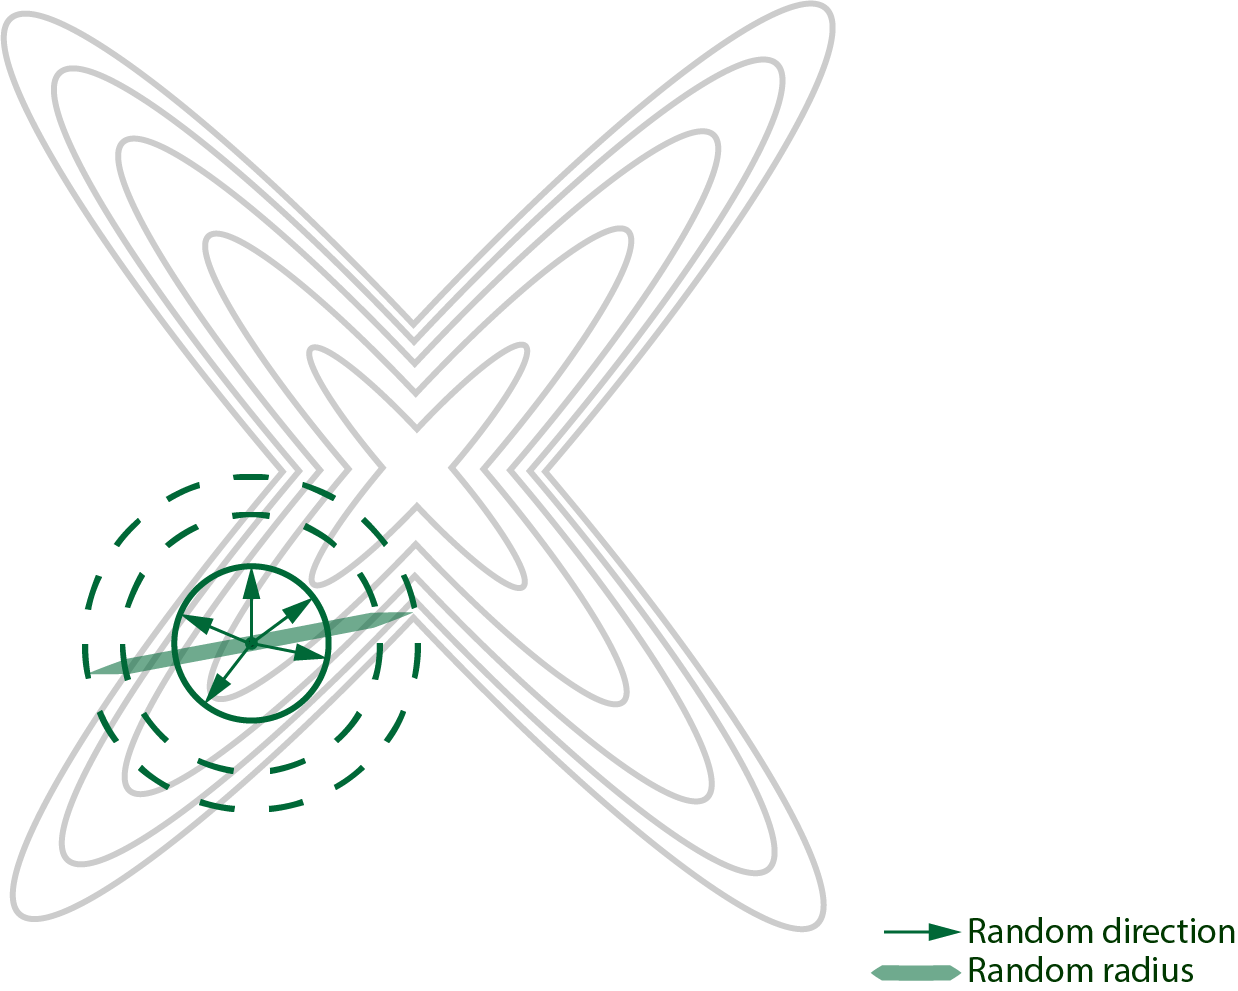
\includegraphics[width=0.5\textwidth]{adaptive-direction}
		\caption{Adaptive direction sampling}
	\end{figure}	
\end{frame}

\begin{frame}
	\frametitle{Resampling from previous samples}
	\begin{itemize}
		\item Re-sampling from previous steps to allow easier movement. \tiny{Atchade, 2006} \normalsize
		\item Arrive at a distribution from re-sampled points that is close to the desired stationary distribution.
	\end{itemize}
	\begin{figure}[h]
		\centering
		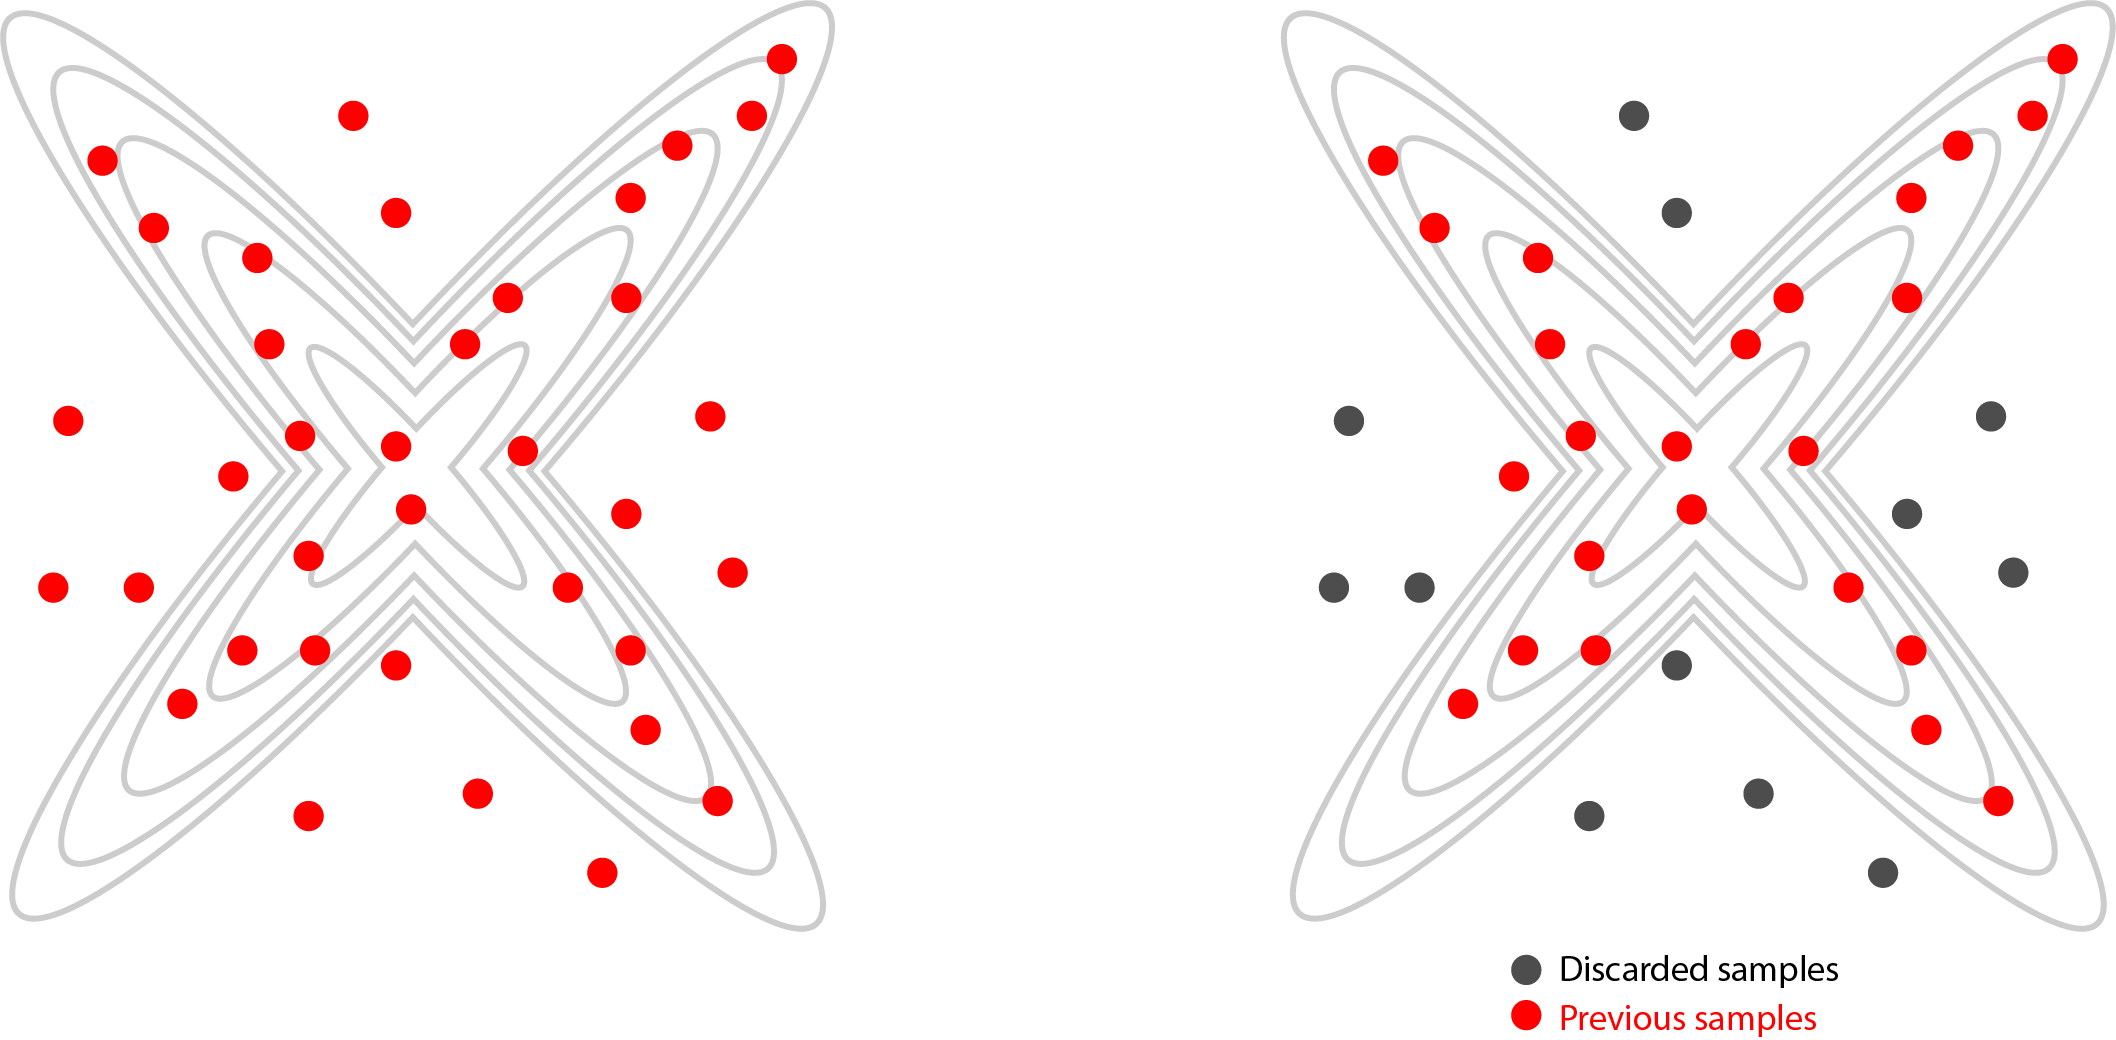
\includegraphics[width=0.8\textwidth]{resampling}
		\caption{Re-sampling from the past steps.}
	\end{figure}	
\end{frame}

\begin{frame}
	\frametitle{Sampling from `easier' distribution}
	\begin{itemize}
		\item Use samples from a different distributions (usually ones we are familiar with.) \tiny{Owen, 2000} \normalsize
		\item Then apply weights to correct over-generation and under-generation.
		\item Cons: Does not work well in high dimensions.
	\end{itemize}
	\begin{figure}[h]
		\centering
		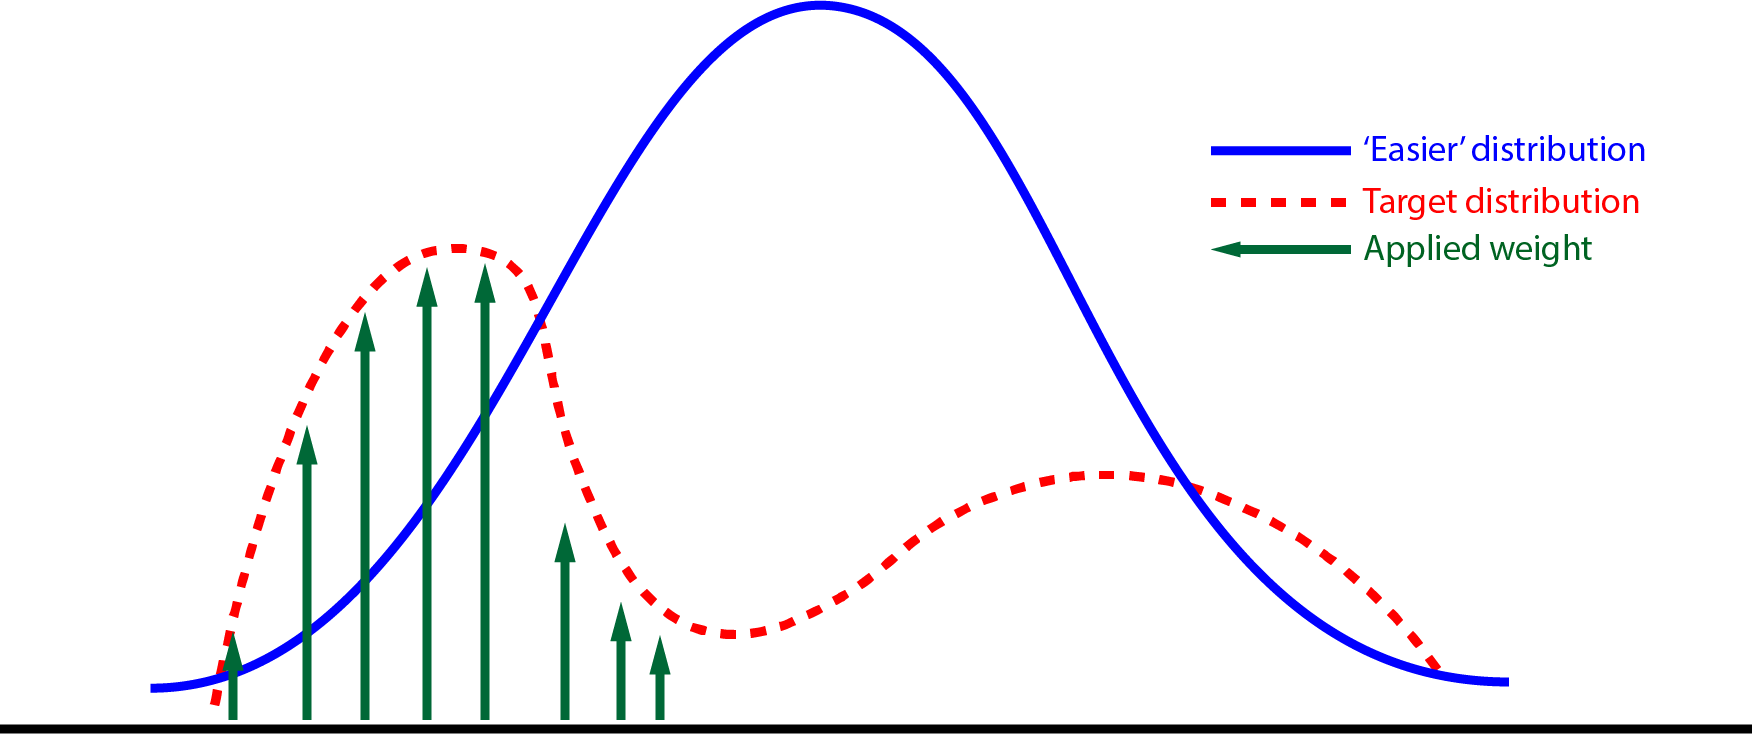
\includegraphics[width=\textwidth]{importance-sampling}
		\caption{Transform the target distribution.}
	\end{figure}	
\end{frame}

\begin{frame}
	\frametitle{(E) Visualising MCMC}
	Code available: \url{https://github.com/quang-ha/mcmc-sampling}
	\centering
		\animategraphics[loop,controls,width=0.63\linewidth]{12}{visualise-}{0}{50}
\end{frame}

\section{Summary}
\begin{frame}[plain]
	\frametitle{Summary}
	\begin{itemize}
		\item It is important for MCMC sampling strategies to achieve rapid mixing, which improves convergence and reduce overall computational cost.
		\item There are several strategies to improve the efficiency of MCMC sampling. The choice of strategy needs careful consideration based on the problem.
		\item There are no global method to check for convergence in MCMC - different attempts have been proposed such as checking autocorrelation function, Gelman-Rubin etc.
	\end{itemize}
\end{frame}
	
\end{document}